\begin{figure*}[t!]
	\begin{center}
		\begin{tabular}{c}
		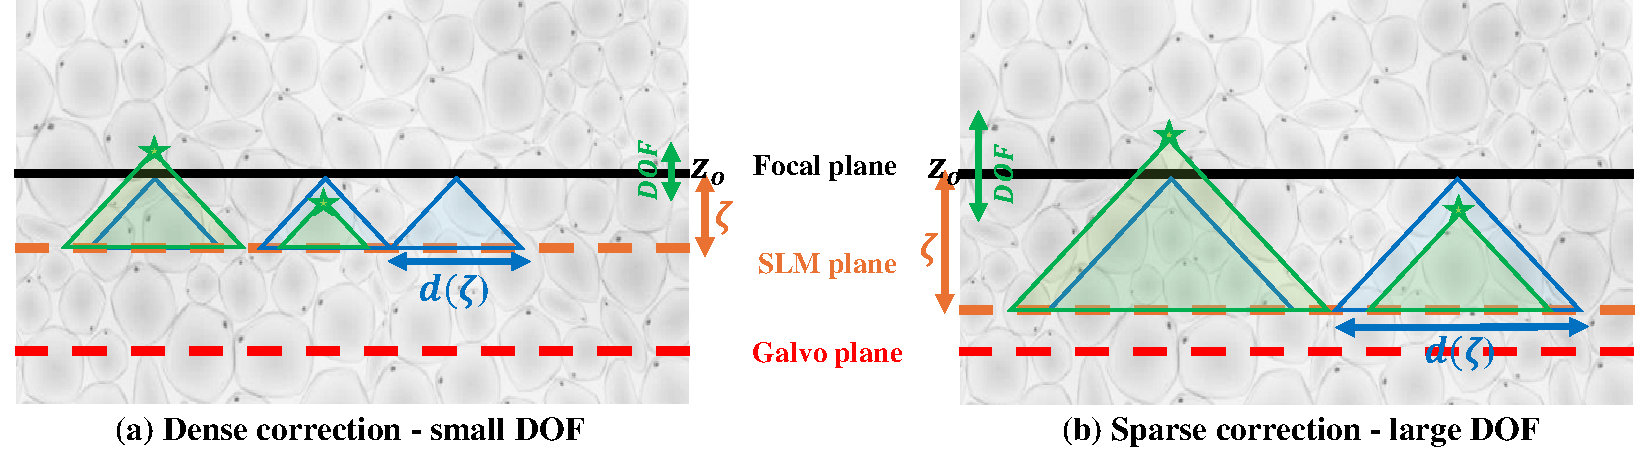
\includegraphics[width= 0.8\textwidth]{figs/system/DOF.pdf}
		%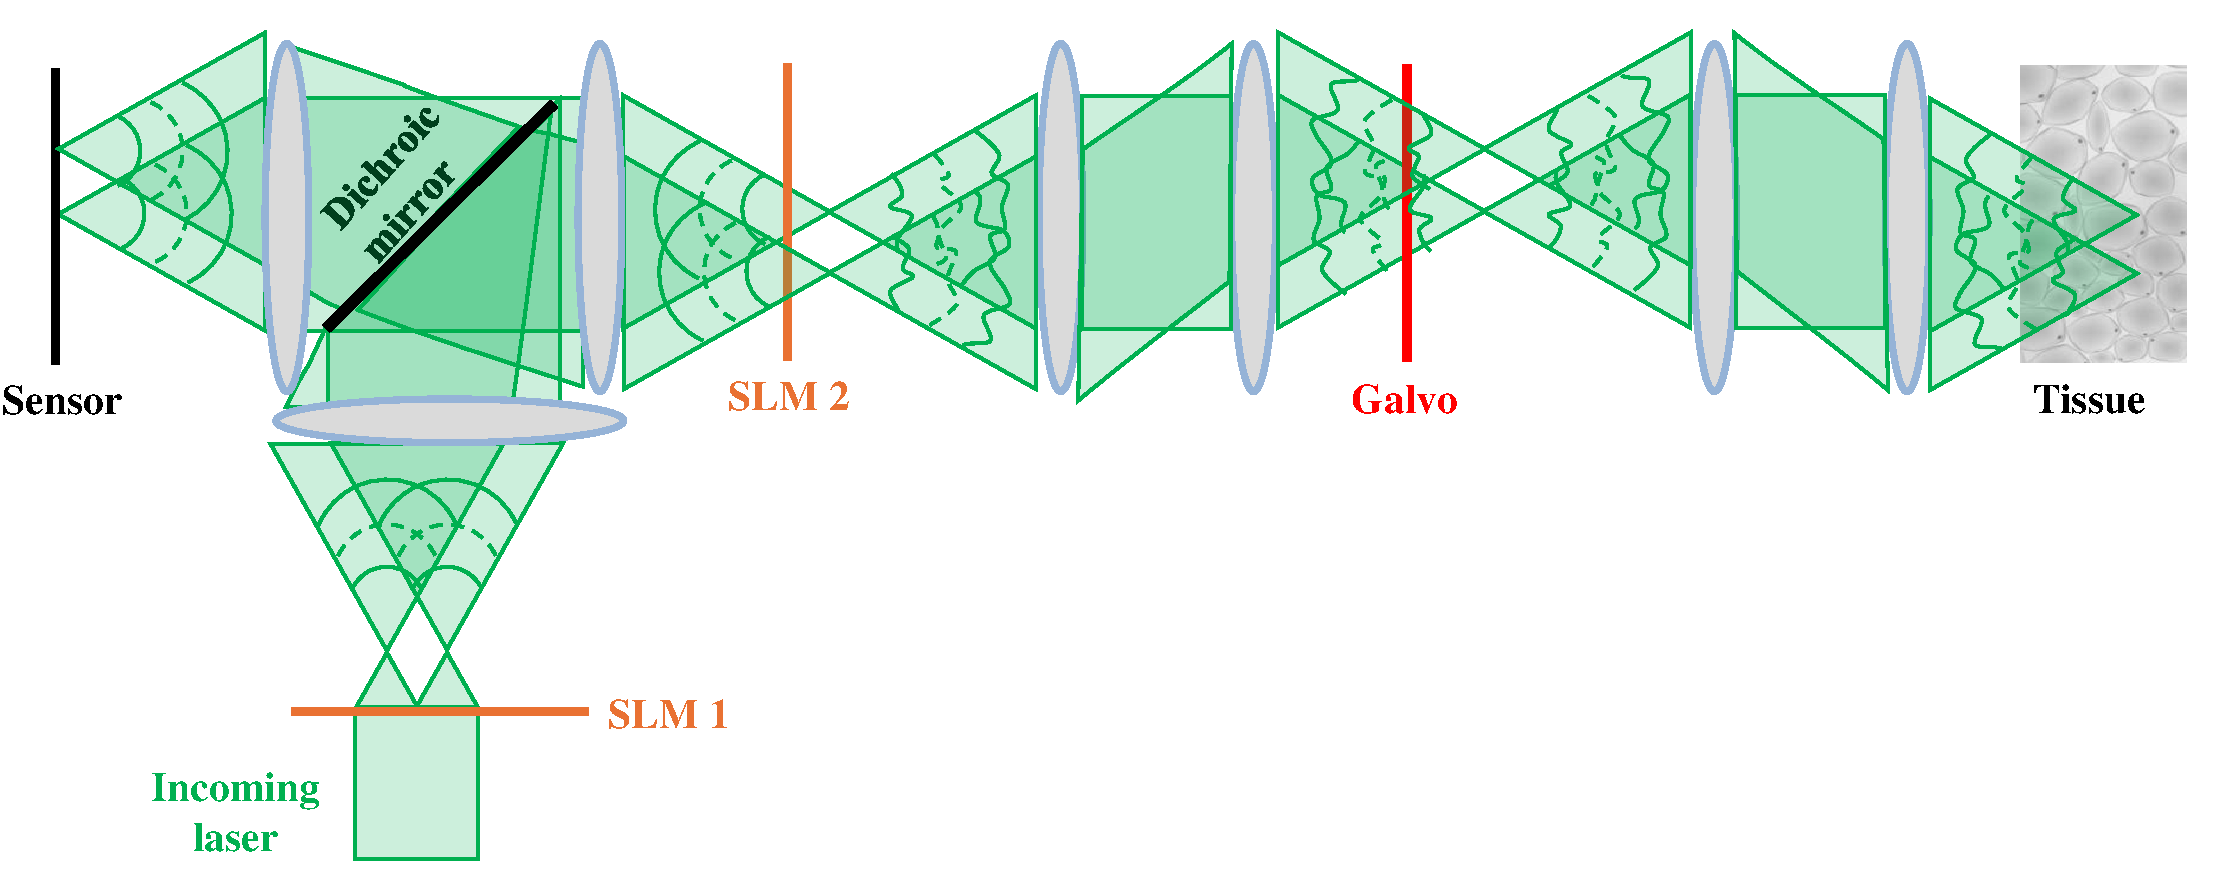
\includegraphics[width= 0.48\textwidth]{figs/system/oneP.pdf}\\
		%(a) Two photon&(b) One photon
		\end{tabular}
	\end{center}
	\caption{{\bf{Depth of field vs. sparsity:}} We visualize the conjugate position of the SLM modulation and the galvo tilt inside the brain tissue.  The distance of the SLM plane from the focal plane controls the diameter of defocus footprint from each target neuron. This diameter should be at least as large as the number of aberration modes one wish to correct. Increasing the distance allows more tolerance to depth variations of the target neurons, but as more SLM pixels are included in the footprint of each neuron, a sparser set of target neurons can be imaged. In the figure, blue triangles mark the idealized defocus blur of points on the focal point, and green triangles mark defocus footprint of sources at other depths.   } 

\label{fig:dof}
\end{figure*}

